%% -*- eval: (flyspell-mode 1); -*-

\documentclass[a4paper,10pt]{article}
\usepackage[utf8]{inputenc}
\usepackage[T1]{fontenc}
\usepackage[french]{babel}
\usepackage{eso-pic}
\usepackage{calc}

\usepackage{graphicx}
\graphicspath{{./img/}}

\usepackage{tikz}
\usetikzlibrary{arrows,positioning,fit}

\usepackage{color}
\usepackage{enumitem}
\usepackage{amsmath}
\usepackage{minted}
\usepackage[tikz]{bclogo}
\usepackage[a4paper,right=2cm]{geometry}

%Sans serif font
\renewcommand{\familydefault}{\sfdefault}

%Header parameters
\newcommand{\subject}{Développement d'un DSEL pour optimiser les calculs sur les stencils}
\newcommand{\intern}{Alexandre Honorat (PRCD)}
\newcommand{\tutor}{Olivier Aumage et Denis Barthou}
\newcommand{\companyname}{INRIA Bordeaux -- équipe Storm}

%% put prend les longueurs sans unités d'où ce petit code :
\makeatletter
\newcommand*{\getlength}[1]{\strip@pt#1}
% Or rounded back to `cm` (there will be some rounding errors!)
%\newcommand*{\getlength}[1]{\strip@pt\dimexpr0.035146\dimexpr#1\relax\relax}
\makeatother

\AddToShipoutPictureBG*{
%% background
  \AtPageUpperLeft{\raisebox{-\height}{\includegraphics[width=\paperwidth,height=\paperheight]{Modele_Poster_A4.eps}}}

%% logo écoles à gauche
  \AtPageUpperLeft{\put(30,-30){\raisebox{-\height}{\includegraphics[width=5cm]{bx-inp-vecto.eps}}}}
  \AtPageLowerLeft{\put(30,30){\includegraphics[width=5cm]{em-bxinp.eps}}}

%% vos logos à droite (exemple avec ceux de l'école)
\newlength{\mylengthLogo}
\setlength{\mylengthLogo}{\paperwidth - 6cm - 30pt}
\newlength{\mylengthImg}
\setlength{\mylengthImg}{\paperwidth - 3cm - 30pt}
%%\def\unitlength{}
  \AtPageUpperLeft{{\put(\getlength{\mylengthImg},-30){\raisebox{-\height}{\includegraphics[width=3cm]{moi.jpg}}}}}
  \AtPageLowerLeft{\put(\getlength{\mylengthLogo},45){\includegraphics[width=6cm]{INRIA_sc.png}}}

%% minipage de titre
\newlength{\mylengthTitre}
\setlength{\mylengthTitre}{0.25\paperwidth + 0.8cm}
  \AtPageUpperLeft{{\put(\getlength{\mylengthTitre},-60){\raisebox{-\height}{
	\begin{minipage}[b]{0.5\paperwidth}
		\centering
		{\LARGE \textbf{\subject}}
                \end{minipage}
        }
    }}}
}


\pagestyle{empty}

\begin{document}

\begin{center}

\vspace{0.2cm}

  {\large Stagiaire : \intern}\\
  {\large Encadrants : \tutor}\\
  {\large Entreprise : \companyname}

\vspace{0.25cm}

\begin{bclogo}[couleur=black!10,couleurBord=black!50,arrondi=0.1,logo=\hspace{17pt},barre=none]{Objectifs du stage}
Le stage effectué avait pour but la conception d'un \emph{DSEL} (Domain Specific Embedded Language) destiné à faciliter l'écriture et la parallélisation de codes à base de stencils. Deux aspects ont donc été étudiés : la sémantique du DSEL (quelles informations il doit être capable de comprendre) et les performances (obtenues par la parallélisation sur carte graphique notamment).

Concrètement un stencil est le calcul d'un élément d'un tableau grâce à ses voisins, comme illustré ci-dessous par une représentation graphique et la formule mathématique associée. Le cas le plus simple serait par exemple : $A[i] = 1.0 \times A[i+1]$.

\begin{minipage}[c]{0.6\textwidth}
\begin{equation*}
\begin{aligned}
g(i,j,B) = & f(i, j, -1, \quad 0, C) \otimes g(i-1, j+0, A) \, \oplus \\
           & f(i, j, \quad 1, \quad 0, C) \otimes g(i+1,j+0, A) \, \oplus \\
           & f(i, j, \quad 0, -1, C) \otimes g(i+0,j-1, A) \, \oplus \\ 
           & f(i, j, \quad 0, \quad 1, C) \otimes g(i+0,j+1, A)
\end{aligned}
\end{equation*}
\end{minipage}%
\begin{minipage}[c]{.3\textwidth}
\begin{tikzpicture}[scale=0.6]
\tikzstyle{place}=[circle,thick,draw=blue!75,fill=blue!20,minimum size=4mm]

\node[place] (p1) at (0,0) {};
\node[place] (p2) at (0,1) {};
\node[place] (p3) at (1,0) {};
\node[place] (p4) at (-1,0) {};
\node[place] (p5) at (0,-1) {};

\node[place] () at (-1,-1) {};
\node[place] () at (-1,1) {};
\node[place] () at (1,-1) {};
\node[place] () at (1,1) {};

\draw[->,thick] (p2) to (p1);
\draw[->,thick] (p3) to (p1);
\draw[->,thick] (p4) to (p1);
\draw[->,thick] (p5) to (p1);

\tikzstyle{place}=[circle,thick,draw=red!75,fill=red!20,minimum size=4mm]

\foreach \x in {-2,...,2}
{
  \node[place] () at (\x,2) {};
  \node[place] () at (\x,-2) {};
  \node[place] () at (2,\x) {};
  \node[place] () at (-2,\x) {};
}



\end{tikzpicture}

\end{minipage}%

Équation générale du stencil à $4$ points en deux dimensions, A est le tableau d'entrée, B celui de sortie, C celui des coefficients. $f$ et $g$ sont des fonctions d'accès aux tableaux. $i,j$ est l'indice courant, $-1,0$ l'indice relatif d'un voisin. Les éléments en rouge sur l'image de droite sont \emph{fantômes} : le stencil ne peut pas leur être appliqué mais ils sont utilisés pour les mises à jour des éléments internes.

\end{bclogo}

\vspace{0.15cm}

\begin{bclogo}[couleur=black!10,couleurBord=black!50,arrondi=0.1,logo=\hspace{17pt},barre=none]{Réalisation : implantation en C++14 et reposant sur triSYCL}
\textsf{SYCL} est une interface de parallélisation en cours de normalisation, elle permettra de gérer simplement tout type de processeur et s'occupera automatiquement des chargements mémoires. \textsf{triSYCL} en est le prototype développé par Ronan Keryell, et utilisé dans le DSEL. Ci-dessous un exemple de code utilisant le DSEL pour le stencil ci-dessus, et le processus général à appliquer (en bleu).

\begin{minipage}[c]{0.55\textwidth}
\begin{minted}[frame=single]{cpp}
coef_fxd2D<0, -1> c1 {1.0};
coef_fxd2D<1, 0> c2 {1.0};
coef_fxd2D<0, 1> c3 {1.0};
coef_fxd2D<-1, 0> c4 {1.0};
auto st = c2+c3+c4+c5;
input_fxd2D<float, &ioABuffer, &fdl_in> 
  work_in;
output_2D<float, &ioBuffer, &fdl_out> 
  work_out;
auto op_work = work_out << st << work_in;
\end{minted}
\end{minipage}%
\begin{minipage}[c]{0.45\textwidth}
\textcolor{blue}{
\begin{enumerate}[itemsep=-1mm]
\item $\Rightarrow$ initialiser les coefficients ;
\item $\Rightarrow$ les assembler pour former un stencil ;
\item déclarer et initialiser les tableaux avec \textsf{SYCL} qui gère les transferts mémoire ;
\item $\Rightarrow$ regrouper les informations nécessaires au calcul (stencil, tableaux et fonctions) au sein d'objets \emph{input} et \emph{output};
\item $\Rightarrow$ créer l'\emph{operation} à partir du stencil, \emph{input} et \emph{output} ;
\item déclarer une queue de calcul avec \textsf{SYCL} ;
\item appeler la méthode de lancement des calcul sur l'objet \emph{operation}.
\end{enumerate}
}
\end{minipage}

Le DSEL est codé en \textsf{C++14} afin de bénéficier des \textsf{lambdas fonctions}, du type \textsf{auto}. Il s'appuie sur les \emph{templates} et la spécialisation partielle pour sélectionner les implantations les plus adaptées aux machines (par exemple le \emph{tiling} pour les GPU) et pour calculer des paramètres à la compilation.

\end{bclogo}

\vspace{0.15cm}

\begin{bclogo}[couleur=black!10,couleurBord=black!50,arrondi=0.1,logo=\hspace{17pt},barre=none]{Conclusion}
Alors qu'un code écrit en \textsf{OpenCL} pour le stencil à $4$ points présenté nécessite $177$ lignes, le DSEL n'en demande que $42$. Les performances sémantiques sont donc au rendez-vous, il reste toutefois beaucoup d'améliorations possibles, notamment pour les techniques de parallélisation utilisées.

\end{bclogo}

\end{center}

\end{document}
